\documentclass[11pt,colorlinks=true]{article}
\usepackage[margin=3cm]{geometry}



\usepackage[utf8x]{inputenc}
\usepackage[english,russian]{babel}
\usepackage{cmap}

\usepackage{amsmath}
\usepackage{amsthm}
\usepackage{bm}
\usepackage{bbold}
\usepackage{amssymb}

\usepackage{graphicx}


\usepackage{hyperref}


\DeclareMathOperator{\T}{T}
\DeclareMathOperator{\tr}{tr}
\DeclareMathOperator{\Tr}{Tr} 
\DeclareMathOperator{\MSE}{MSE} 
\DeclareMathOperator{\E}{E}
\DeclareMathOperator{\D}{D}

\newtheorem{theorem}{Теорема}
\newtheorem{lemma}{Лемма}
\newtheorem{corollary}{Следствие}
\newtheorem{statement}{Утверждение}
\newtheorem{note}{Замечание}
\newtheorem{theorem+}{Теорема Гаусса-Маркова}
\newtheorem{proposition}{Предложение}

\begin{document}

	\thispagestyle{empty}
%
	\begin{center}
		Санкт-Петербургский государственный университет \\
		\vspace{0.3cm}	
		Прикладная математика и информатика \\
		\vspace{0.3cm}
		Кафедра статистического моделирования \\
		
		\vspace{6cm}			   	
			
			\vspace{0.3cm}	
			%\vspace{2cm}	
			 {\huge Регрессия и регуляризация} \\
			 \vspace{0.5cm}
									Романова Елизавета \\
			Горбачук Анна \\
			Сидоренко Денис \\

			\vspace{10cm}	

		Санкт-Петербург \\
				2019
	\end{center}
	
\newpage


\tableofcontents

\newpage

\section{Обучение с учителем}

Пусть наблюдается некоторый количественный отклик $Y$ и $p$ предикторов (признаков) $X_{1},\ldots,X_{p}$. 
Будем предполагать, что между $Y$ и $X=(X_{1},\ldots,X_{p})$ существует определенная связь, которую можно представить в виде
\begin{equation*}
Y
=
f^{\ast}(X)+\varepsilon,
\end{equation*}
где $f^{\ast}$ --- фиксированная, но неизвестная функция от предикторов, $\varepsilon$ --- ошибка, которая не зависит от $X$ и имеет нулевое среднее значение.

Можно рассматривать две различные задачи с разными целями: предсказание (prediction) и статистический вывод (inference).

\begin{itemize}
\item \textbf{Prediction.}

Так как ошибки имеют нулевое среднее, можем предсказывать $Y$ в соответствии с формулой 
\begin{equation*}
\hat{Y}
=
\hat{f}(X),
\end{equation*}
где $\hat{f}$ --- оценка $f^{\ast}$, $\hat{Y}$ --- предсказанное значение $Y$.

Когда целью является предсказание, нам не важна точная форма функции $\hat{f}$, если она обеспечивает точные предсказания $Y$.
\item\textbf{ Inference.}

Интересуемся тем, как изменения $X_{1},\ldots,X_{p}$ влияют на $Y$. То есть, цель --- оценить $f^{\ast}$ (а не предсказать $Y$). В таком случае нужно знать точную форму $\hat{f}$.
\end{itemize}

В настоящем курсе нас больше интересуют предсказания.

Пусть имеется выборка из $n$ отдельных наблюдений: $x_{1},\ldots,x_{n}$ для которых известны соответствующие значения отклика. Обозначим $x_{ij}$ --- значение $j$-го признака $i$-го наблюдения, $x_{i}=(x_{i1},\ldots,x_{ip})^{\T}$,  $y_{i}$ --- отклик у $i$-го наблюдения.
 
 Хотим найти такую функцию $\hat{f}$, что $y\approx\hat{f}(x)$ для любого наблюдения $(x,y)$.  
 Совокупность $X_{n}$ пар $(x_{1}, y_{1}),\ldots, (x_{n},y_{n})$, которая участвует в оценке функции $f^{\ast}$, называется обучающей выборкой.
 Выборка $X_{k}^{\prime}=(x_{i}^{\prime},y_{i}^{\prime})_{i=1}^{k}$, не участвующая в оценке функции $f^{\ast}$, называется тестовой (или контрольной).

\section{Регрессия}

 
 \subsection{Регрессия и МНК}
 
Итак, пусть дана обучающая выборка $X_{n}=(x_{i},y_{i})_{i=1}^{n}$, где $x_{i}\in\mathbb{R}^{p}$, $y_{i}\in\mathbb{R}$ и предполагается, что между ответами и объектами есть связь:
\begin{equation*}
y_{i}=f^{\ast}(x_{i})+\varepsilon_{i},
\qquad 
i=1,\ldots,n.
\end{equation*}
где $\varepsilon_{i}$ --- независимые одинаково распределенные случайные величины с $\E\varepsilon_{i}=0$, $\E\varepsilon_{i}^{2}=\sigma^{2}$.

Пусть задана модель регрессии --- параметрическое семейство функций $f(x,\theta)$, где $\theta\in\Theta$ --- вектор параметров модели, $\Theta\subset\mathbb{R}^{p}$ --- пространство параметров,
$f:\mathbb{R}^{p}\times\Theta\rightarrow\mathbb{R}$ --- фиксированная функция.
Выберем в качестве функционала качества аппроксимации целевой зависимости на выборке $X_{n}$ среднеквадратическую ошибку:
\begin{equation}\label{eq:MSE}
\MSE_{\text{train}}
=
Q(\theta,X_{n})=
\frac{1}{n}
\sum_{i=1}^{n}
(f(x_{i},\theta)-y_{i})^{2}.
\end{equation}

Обучение по методу наименьших квадратов (МНК) состоит в нахождении такого вектора параметров $\theta^{\ast}$, при котором достигается минимум среднего квадрата ошибки на заданной обучающей выборке $X_{n}$:
\begin{equation*}
\theta^{\ast}=
\arg\min_{\theta\in\mathbb{R}^{p}}
Q(\theta,X_{n}).
\end{equation*}

$\MSE$ в \eqref{eq:MSE} вычисляется на основе обучающей выборки, то есть наблюдений, которые были использованы для подгонки модели, так что это ошибка на обучающей выборке. В реальности нас интересует ошибка $\MSE$ на контрольной выборке, то есть то, насколько метод дает точное предсказание для наблюдений, которые не участвовали в оценке $f^{\ast}$. 
Нет гарантии, что метод с минимальной среднеквадратической ошибкой на обучающих данных также будет иметь минимальную $\MSE$ на контрольных данных.

Когда качество работы алгоритма на новых объектах, не вошедших в состав обучения, оказывается существенно хуже, чем на обучающей выборке ($\mathrm{MSE_{\text{test}}}\gg\mathrm{MSE}_{\text{train}}$), говорят об эффекте переобучения (overtraining) или переподгонки (overfitting).

\subsection{Bias–variance tradeoff}

Пусть $(x^{\prime},y^{\prime})\in X_{k}^{\prime}$ --- объект данных из тестовой выборки, $y^{\prime}=f^{\ast}(x^{\prime})+\varepsilon$, $\E\varepsilon=0$, $\E\varepsilon^{2}=\sigma^{2}$. 

Для математического ожидания квадрата ошибки предсказания на $(x^{\prime},y^{\prime})$ справедливо
\begin{equation}\label{eq:MSE_test_y}
\E(\hat{f}(x^{\prime})-y^{\prime})^{2}
=
\D\hat{f}(x^{\prime})+(\mathrm{Bias}\hat{f}(x^{\prime}))^{2}+\sigma^{2},
\end{equation}
$\D\hat{f}$ --- дисперсия оценки $\hat{f}$, $\mathrm{Bias}\hat{f}(x^{\prime})$ --- смещение оценки, $\sigma^{2}$ --- неустранимая ошибка.

%(Эта формула интересна в контексте prediction)

В контексте inference нас может больше интересовать аналогичная формула 
\begin{equation}\label{eq:MSE_test_f}
\E(\hat{f}(x^{\prime})-f^{\ast}(x^{\prime}))^{2}
=\D\hat{f}(x^{\prime})+(\mathrm{Bias}\hat{f}(x^{\prime}))^{2}.
\end{equation}

Таким образом, $\MSE$ на контрольной выборке зависит от дисперсии оценки и квадрата ее смещения.
Дисперсия оценки определяет то количество, на которое изменится $\hat{f}$, если бы мы получали эту оценку с использованием другого набора данных. Мы хотим, чтобы оценка $\hat{f}$ не менялась сильно на разных обучающих выборках. Смещение $\hat{f}$ характеризует ошибку, возникающую при аппроксимации реальной сложной функции $f^{\ast}$ более простой моделью. То есть для минимизации ожидаемой ошибки на контрольных данных нужен такой метод обучения, который обеспечивает и низкую дисперсию, и низкое смещение.

\subsection{Множественная линейная регрессия}
Предполагаем, что зависимость между ответами и признаками линейная, а также, что ответы и признаки центрированы (для краткости записи: чтобы не приходилось дописывать свободный член или добавлять в матрицу $\mathbb{X}$ столбец из единиц).

Модель множественной линейной регрессии ($\beta_{1},\ldots,\beta_{p}$ --- параметры модели):
\begin{equation*}
y_{i}
=
f(x_{i}; \beta_{1},\ldots,\beta_{p})+\varepsilon_{i}
=
\sum_{j=1}^{p}\beta_{j}x_{ij}+\varepsilon_{i}.
\end{equation*}

Введем матричные обозначения:
\begin{equation*}
\mathbb{X}=[X_{1}:\ldots:X_{p}]=
\begin{pmatrix}
x_{11} &x_{12} &\ldots &x_{1p}\\
x_{21} &x_{22} &\ldots &x_{2p}\\
\vdots &\vdots &\ddots &\vdots\\
x_{n1} &x_{n2} &\ldots &x_{np}
\end{pmatrix},
\quad
Y
=
\begin{pmatrix}
y_{1}\\
y_{2}\\
\vdots\\
y_{n}
\end{pmatrix},
\quad
B=
\begin{pmatrix}
\beta_{1}\\
\beta_{2}\\
\vdots\\
\beta_{p}
\end{pmatrix},
\quad
\mathcal{E}
=
\begin{pmatrix}
\varepsilon_{1}\\
\varepsilon_{2}\\
\vdots\\
\varepsilon_{n}
\end{pmatrix}.
\end{equation*}



Модель множественной линейной регрессии в матричной записи: 
\begin{equation*}
Y=\mathbb{X}B+\mathcal{E}.
\end{equation*}

Минимизируем среднеквадратическую ошибку 
\begin{equation*}
Q(B,X)
=
\frac{1}{n}
\sum_{i=1}^{n}
\left(
y_{i}-
\sum_{j=1}^{p}\beta_{j}x_{ij}
\right)^{2}
=
\frac{1}{n}
||Y-\mathbb{X}B||^{2}
=
\frac{1}{n}
(Y-\mathbb{X}B)^{\mathrm{T}}(Y-\mathbb{X}B)
\rightarrow
\min_{B}.
\end{equation*}

Решение МНК:
\begin{equation}\label{eq:olsB}
\hat{B}=(\mathbb{X}^{\mathrm{T}}\mathbb{X})^{-1}\mathbb{X}^{\mathrm{T}}Y=\mathbb{X}^{-}Y,
\qquad
\hat{Y}=\mathbb{X}\hat{B}.
\end{equation}


Вычислительная проблема:  при плохой обусловленности матрицы $\mathbb{X}^{\mathrm{T}}\mathbb{X}$ вычисление обратной к ней матрицы крайне нежелательно. Поэтому на практике лучше избегать прямого использования формул \eqref{eq:olsB}.

\textbf{Варианты обхода:}
\begin{itemize}
\item Переход к нормальной системе ($p$ неизвестных, $p$ уравнений):
\begin{equation*}
\mathbb{X}^{\mathrm{T}}Y=
\mathbb{X}^{\mathrm{T}}\mathbb{X}B.
\end{equation*}
Существует большое количество численных методов решения нормальной системы. Наибольшей популярностью пользуются методы, основанные на ортогональных
разложениях матрицы $\mathbb{X}$ ($QR$-разложение, например). Эти методы эффективны, обладают хорошей численной устойчивостью и позволяют строить различные модификации и обобщения.
\item Использование сингулярного разложения.

Пусть $\mathbb{X}=\mathbb{V}\mathbb{\Lambda}\mathbb{U^{\mathrm{T}}}$ --- сингулярное разложение $\mathbb{X}$.
Тогда псевдообратную к $\mathbb{X}$ матрицу легко записать в виде
\begin{equation*}
\mathbb{X}^{-}
=
\mathbb{U}\mathbb{\Lambda}^{-1}\mathbb{V}^{\mathrm{T}}
=
\sum_{j=1}^{p}
\frac{1}{\sqrt{\lambda_{j}}}
U_{j}V_{j}^{\mathrm{T}}.
\end{equation*}
Вектор МНК-решения:
\begin{equation}\label{eq:B_SVD}
\hat{B}=\mathbb{X}^{-}Y
=
\sum_{j=1}^{p}
\frac{1}{\sqrt{\lambda_{j}}}
U_{j}(V_{j}^{\mathrm{T}}Y).
\end{equation}
Оценка $Y$:
\begin{equation}\label{eq:Y_SVD}
\hat{Y}
=
\mathbb{X}\hat{B}
=
\sum_{j=1}^{p}
V_{j}(V_{j}^{\mathrm{T}}Y).
\end{equation}
Норма вектора коэффициентов:
\begin{equation}\label{eq:||B||_SVD}
||\hat{B}||^{2}
=
\sum_{j=1}^{p}
\frac{1}{\lambda_{j}}(V_{j}^{\mathrm{T}}Y)^{2}.
\end{equation}
Таким образом, имея сингулярное разложение, не приходится вычислять обратную матрицу. Эффективные численные алгоритмы, вычисляющие SVD, реализованы
во многих стандартных математических пакетах.
\end{itemize}


\subsection{Мультиколлинеарность}

Проблема мультиколлинеарности является общей для многих методов корреляционного анализа. МНК не исключение. 

Если матрица данных содержит несколько сильно коррелированных признаков, то есть матрица начинает приближаться к вырожденной, то минимальное собственное число становится близким к $0$.
 Что будет происходить в таком случае с МНК-оценкой? 

При очень малых собственных числах $\lambda_{j}$ соответствующие знаменатели в формулах \eqref{eq:B_SVD} и \eqref{eq:||B||_SVD} близки к нулю. Поэтому в суммах появляются очень большие и неустойчивые слагаемые.

Теряется интерпретируемость оценок коэффициентов (это важно, если нас интересует inference), так как коэффициенты могут неоправданно принимать очень большие значения. 

При этом мы не заметим проблем, работая только с обучающей выборкой, так как на ней $Y$ по-прежнему будет хорошо приближаться (в формуле \eqref{eq:Y_SVD} не участвуют собственные числа). Но на тестовой выборке ответы $Y^{\prime}=\mathbb{X}^{\prime}\hat{B}$  неустойчивы.


Таким образом, в линейных моделях мультиколлинеарность приводит к переобучению.

\textbf{Способы решения проблемы:}
\begin{itemize}
\item Регуляризация: проблема зарождается в мультиколлинеарности, а проявляется в том, что норма вектора коэффициентов увеличивается. Регуляризация контролирует увеличение нормы вектора.
\item Преобразование признаков.
\item Отбор признаков.
\end{itemize}


\section{Регуляризация}

В соответствии с формулами \eqref{eq:MSE_test_y}, \eqref{eq:MSE_test_f}, $\MSE$ на контрольной выборке зависит от дисперсии оценки $\hat{f}$ и ее смещения.

Когда связь между откликом и предикторами (почти) линейна, оценки по методу наименьших квадратов обладают (почти) нулевым смещением, но при этом могут иметь высокую дисперсию. 

Ковариационная матрица МНК-оценки $\hat{B}$: 
\begin{equation}\label{eq:Cov_ols}
\mathrm{Cov}(\hat{B}) = \sigma^2(\mathbb{X}^{\T}\mathbb{X})^{-1}.
\end{equation}
Чем больше дисперсия оценки $\hat{B}$, тем больше дисперсия $\hat{f}$. Когда матрица $\mathbb{X}$ близка к вырожденной (это может произойти из-за наличия мультиколлинеарности или когда число предикторов $p$ почти равно числу наблюдений $n$), дисперсия $\hat{B}$ становится большой и $\mathrm{MSE}_{\mathrm{test}}$ увеличивается.  При $p>n$ или при полностью коллинеарных признаках оценки по методу наименьших квадратов не имеют уникального решения.

Введение небольшого смещения в оценке может привести к значительному уменьшению дисперсии и тем самым уменьшению $\mathrm{MSE}_{\text{test}}$.


\subsection{Регуляризация Тихонова}

Метод наименьших квадратов решает нормальную систему $\mathbb{X}^{\T}\mathbb{X}B=\mathbb{X}^{\T}Y$.
Идея метода регуляризации Тихонова состоит в том, чтобы прибавить к (возможно) плохо обусловленной матрице $\mathbb{X}^{\T}\mathbb{X}$ другую матрицу  $\mathbb{T}^{\T}\mathbb{T}$ так, чтобы их сумма была хорошо обусловлена. Переходим к следующей нормальной системе: 
\begin{equation*}
(\mathbb{X}^{\T}\mathbb{X}+\mathbb{T}^{\T}\mathbb{T})B=\mathbb{X}^{\T}Y.
\end{equation*}

Решение последней системы соответствует минимизации функции 
\begin{equation*}
||Y-\mathbb{X}B||_{2}^{2}+||\mathbb{T}B||_{2}^{2}.
\end{equation*}

Решение: 
\begin{equation*}
\hat{B}_{T}
=(\mathbb{X}^{\T}\mathbb{X}+\mathbb{T}^{\T}\mathbb{T})^{-1}\mathbb{X}^{\T} Y.
\end{equation*}

Оценка $\hat{B}_{T}$, конечно, уже будет иметь смещение:
\begin{equation*}
\E\hat{B}_{T}
=
(\mathbb{X}^{\T}\mathbb{X}+\mathbb{T}^{\T}\mathbb{T})^{-1}\mathbb{X}^{\T}\mathbb{X}B.
\end{equation*}

Легко показать, что ковариационная матрица полученной оценки
\begin{equation*}
\mathrm{Cov}(\hat{B}_{T})
=
\sigma^{2}
(\mathbb{X}^{\T}\mathbb{X}+\mathbb{T}^{\T}\mathbb{T})^{-1}
\mathbb{X}^{\T}\mathbb{X}
((\mathbb{X}^{\T}\mathbb{X}+\mathbb{T}^{\T}\mathbb{T})^{-1})^{\T},
\end{equation*}
поэтому при наличии полностью коллинеарных признаков дисперсия соответствующей оценки $\hat{f}_{\T}$ (и, как следствие, $\MSE_{\text{test}}$) будет конечна, в отличие от дисперсии \eqref{eq:Cov_ols} обычной МНК-оценки \eqref{eq:olsB}.


\subsection{Гребневая регрессия (Ridge regression)}

Гребневая регрессия --- это наиболее распространенный частный случай метода регуляризации Тихонова с $\mathbb{T}=\sqrt{\tau}\mathbb{I}$.

\subsubsection{Задача гребневой регрессии}
Вводится штраф за увеличение нормы вектора $B$ и минимизируется следующая функция:
\begin{equation*}
Q_{\tau}(B)
=
||\mathbb{X}B-Y||^{2}
+
\tau||B||^{2}
\rightarrow\min_{B},
\end{equation*}
где $\tau$ --- неотрицательный параметр регуляризации.

В развернутом виде задача оптимизации записывается так:
\begin{equation*}
\sum_{i=1}^{n}
\left(
y_{i}
-
\sum_{j=1}^{p}\beta_{j}x_{ij}
\right)^{2}
+
\tau\sum_{j=1}^{p}\beta_{j}^{2}
\rightarrow\min_{B}.
\end{equation*}


Решение задачи гребневой регрессии:
\begin{equation*}
\hat{B}_{\tau}
=
(\mathbb{X}^{\mathrm{T}}\mathbb{X}+\tau\mathbb{I}_{p})^{-1}\mathbb{X}^{\mathrm{T}}Y.
\end{equation*}



\subsubsection{Параметр регуляризации}
Чем больше коэффициент регуляризации $\tau$, тем устойчивее решение, но больше смещение. 
Когда $\tau = 0$, гребневая регрессия совпадает с обычной регрессией, но при $\tau \rightarrow \infty$ коэффициенты регрессии стремятся к нулю.
Для каждого значения $\tau$ гребневая регрессия порождает свой оптимальный набор оценок коэффициентов $\hat\beta_{1},\ldots,\hat\beta$.
 Важно подобрать хорошее значение параметра $\tau$, чтобы достичь компромисса между смещением и неустойчивостью. 


 Подход на основе сингулярного разложения $\mathbb{X}=\mathbb{V}\mathbb{\Lambda}\mathbb{U^{\mathrm{T}}}$ позволяет подбирать параметр $\tau$, вычислив SVD только один раз.

Решение гребневой регрессии через SVD:
\begin{equation*}
\hat{B}_{\tau} = \mathbb{U}(\mathbb{\Lambda}^2 +\tau \mathbb{I}_{p})^{-1}\mathbb{\Lambda}\mathbb{V}^{\T}Y 
= \sum_{j=1}^p \frac{\sqrt{\lambda_j}}{\lambda_j + \tau} U_j(V_j^{\T}Y).
\end{equation*}

 Оценка функции $f^{\ast}$ для выборки $X_{n}$ через SVD:
\begin{equation*}
\mathbb{X}\hat{B}_{\tau} = \mathbb{V}\mathbb{\Lambda}\mathbb{U}^{\T}\hat{B}_{\tau} = \mathbb{V} \mathrm{diag}\left(\frac{\lambda_j}{\lambda_j + \tau}\right)\mathbb{V}^{\T}Y = \sum_{j=1}^p \frac{\lambda_j}{\lambda_j + \tau} V_j(V_j^{\T}Y).
\end{equation*}

 Таким образом, необходимо один раз произвести сингулярное разложение матрицы $\mathbb{X}$, а затем несложным образом вычислять вектор оценок параметров для интересующих значений параметра $\tau$. 

Добавление в знаменатель положительного числа $\tau$ приводит к тому, что проблема неустойчивости уходит. 

\subsubsection{Вероятностная интерпретация гребневой регрессии}

Пусть в линейной модели выполнены следующие предположения:
\begin{itemize}
\item ошибки независимы и $\varepsilon_{i}\in N(0,\sigma^{2})$ $\forall i=1,\ldots,n$.
\item вектор параметров $B$ имеет априорное распределение $\pi(B)\stackrel{d}{=}N(\bm{0},\frac{\sigma^{2}}{\tau}\mathbb{I})$.
\end{itemize}

 Пусть $L(X,Y,B)$ --- функция правдоподобия выборки. 
 По теореме Байеса при фиксированном $X$ апостериорное распределение $q(B|X,Y)$ пропорционально $L(X,Y,B)\pi(B)$.

Покажем, что в условии выполненных предположений оценка апостериорного максимума $B$ совпадает с решением гребневой регрессии.

Оценка максимума апостериорной вероятности:
\begin{multline*}
\arg\max_{B}q(B|X,Y)
=
\arg\max_{B}L(X,Y,B)\pi(B)
=\\=
\arg\max_{\beta_{1},\ldots,\beta_{p}}\exp
\left(
-\sum_{j=1}^{n}
\frac{\varepsilon_{j}^{2}}{2\sigma^{2}}
\right)
\exp\left(
-\sum_{i=1}^{p}
\frac{\tau\beta_{i}^{2}}{2\sigma^{2}}\right)
=\\=
\arg\max_{\beta_{1},\ldots,\beta_{p}}\exp
\left(-\sum_{j=1}^{n}
\frac{(y_{j}-\sum_{i=1}^{p}\beta_{i}x_{ij})^{2}}{\sigma^{2}}
\right)
\exp
\exp\left(
-\sum_{i=1}^{p}
\frac{\tau\beta_{i}^{2}}{2\sigma^{2}}\right)
=\\=
\arg\max_{B}
\exp
\left(
-\frac{||Y-\mathbb{X}B||^{2}}{2\sigma^{2}}-\frac{\tau||B||^{2}}{2\sigma^{2}}
\right)
=\\=
\arg\min_{B}
(||Y-\mathbb{X}B||^{2}+\tau||B||^{2}).
\end{multline*}

Пришли к решению задачи гребневой регрессией с параметром регуляризации $\tau$.
 

\subsubsection{Проблемы и замечания}
\begin{itemize}
\item Стандартные МНК-оценки инварианты относительно умножения признака на константу, то есть значение $X_{j}\hat{\beta_j}$ не зависит от масштаба $j$-го признака. Оценки МНК гребневой регрессии не обладают свойством инвариантности и могут существенно меняться.
Поэтому гребневую регрессию нужно использовать после стандартизации признаков.
\item  В конечную модель входят все начальные признаки, если признаков много, то усложняется интерпретация.
\end{itemize}





\subsection{Лассо (Lasso)}

С задачей отбора признаков справляется Лассо регрессия, в которой в качестве штрафа на норму коэффициентов используется $l_{1}$-норма вектора коэффициентов.


\subsubsection{Задача Lasso-регрессии}

Метод LASSO решает следующую задачу минимизации:
\begin{equation*}
||\mathbb{X}B-Y||_{2}^{2}
+
\tau||B||_{1}^{2}
\rightarrow\min_{B},
\end{equation*}
где $\tau$ --- неотрицательный параметр регуляризации.

Задача оптимизации в развернутом виде:
\begin{equation*}
\sum_{i=1}^{n}
\left(
y_{i}
-
\sum_{j=1}^{p}\beta_{j}x_{ij}
\right)^{2}
+
\tau\sum_{j=1}^{p}|\beta_{j}|
\rightarrow\min_{\beta_{1},\ldots,\beta_{p}}.
\end{equation*}

Сложность задачи состоит в ее негладкости, из-за которой мы не можем сразу применить теорему~\ref{th:CT} (теорему Куна-Таккера).

 Задачу lasso-оптимизации можно переписать в форме с ограничениями: %(метод множителей Лагранжа)
\begin{equation*}%\label{eq:lasso_constr}
\begin{cases}
\sum_{i=1}^{n}
\left(
y_{i}
-
\sum_{j=1}^{p}\beta_{j}x_{ij}
\right)^{2}
\to
\min_{\beta_{1},\ldots,\beta_{p}},\\
\sum_{j=1}^{p}|\beta_{j}|\leq\ae,
\end{cases}
\end{equation*}
где $\ae=1/\tau$.

Приведем задачу к каноничному виду. Представим каждый параметр $\beta_{j}$ в виде разности положительной и отрицательной частей: $\beta_{j}=\beta_{j}^{+}-\beta_{j}^{-}$. Тогда $|\beta_{j}|=\beta_{j}^{+}+\beta_{j}^{-}$. После замены переменных переходим к задаче 
($2p$ переменных, $2p+1$ ограничений):
\begin{equation*}
\begin{cases}
\sum_{i=1}^{n}
\left(
y_{i}
-
\sum_{j=1}^{p}(\beta_{j}^{+}-\beta_{j}^{-})x_{ij}
\right)^{2}
\to
\min_{\beta_{1}^{+},\ldots,\beta_{p}^{+},\beta_{1}^{-},\ldots,\beta_{p}^{-}},\\
\sum_{j=1}^{p}\beta_{j}^{+}+\beta_{j}^{-}\leq\ae,
\quad
\beta_{j}^{+}\geq 0,
\quad
\beta_{j}^{-}\geq 0.
\end{cases}
\end{equation*}

Получили выпуклую задачу квадратичного программирования с линейными ограничениями-неравенствами, к которой применима теорема Куна-Таккера.

Чем меньше параметр $\ae$, тем больше ограничений обращаются в равенства: $\beta_{j}^{+}=\beta_{j}^{-}=0$, что соответствует обнулению коэффициента $\beta_{j}$ и исключению $j$-го признака.

\subsubsection{Вероятностная интерпретация Лассо}

Пусть в линейной модели выполнены следующие предположения:
\begin{itemize}
\item ошибки независимы и $\varepsilon_{i}\in N(0,\sigma^{2})$ $\forall i=1,\ldots,n$.
\item вектор параметров $B$ имеет априорное распределение $\pi(B)=\prod_{j=1}^{p}g(\beta_{j})$, где $g$ --- плотность распределения Лапласа $\mathrm{Laplace}(0,\tau)$.
\end{itemize}

 Пусть $L(X,Y,B)$ --- функция правдоподобия выборки. %=\prod_{i=1}^{n}p(x_{i},y_{i},B)$. 
 По теореме Байеса при фиксированном $X$ апостериорное распределение $q(B|X,Y)$ пропорционально $L(X,Y,B)\pi(B)$.

В условии выполненных предположений оценка апостериорного максимума $B$ совпадает с решением лассо-регрессии.

\subsection{Сравнение гребневой регрессии и Лассо}

Сначала заметим, что задачу гребневой регрессии можно  представить в виде задачи минимизации с ограничениями
\begin{equation*}
\begin{cases}
\sum_{i=1}^{n}
\left(
y_{i}
-
\sum_{j=1}^{p}\beta_{j}x_{ij}
\right)^{2}
\to
\min_{\beta_{1},\ldots,\beta_{p}},\\
\sum_{j=1}^{p}\beta_{j}^{2}\leq\ae.
\end{cases}
\end{equation*}


Ранее мы также получали соответствующую форму записи для лассо-регрессии:
\begin{equation*}%\label{eq:lasso_constr}
\begin{cases}
\sum_{i=1}^{n}
\left(
y_{i}
-
\sum_{j=1}^{p}\beta_{j}x_{ij}
\right)^{2}
\to
\min_{\beta_{1},\ldots,\beta_{p}},\\
\sum_{j=1}^{p}|\beta_{j}|\leq\ae.
\end{cases}
\end{equation*}

Рассмотрим простой случай, когда $p = 2$. Тогда выражение $\sum_{i=1}^n(y_i - \sum_{j=1}^p \beta_j x_{ij})^2$ --- это эллипс с центром в точке $\hat{B}$. Предположим, что центр эллипса не удовлетворяет ограничениям $\sum_{j = 1}^p \beta_j^2 \leq\ae$ и $\sum_{j = 1}^p |\beta_j| \leq \ae$, то есть лежит вне круга в случае гребневой регрессии и вне ромба в случае Лассо. Тогда решения задач минимизации будут лежать на границе возможных значений. На рис.~\ref{lasso_pic} видно, что для Лассо существует гораздо больше различных эллипсов, которые пересекались бы с ромбом (ограничениями) таким образом, чтобы один из коэффициентов был равен нулю.

\begin{figure}[h]
\label{lasso_pic}
\center{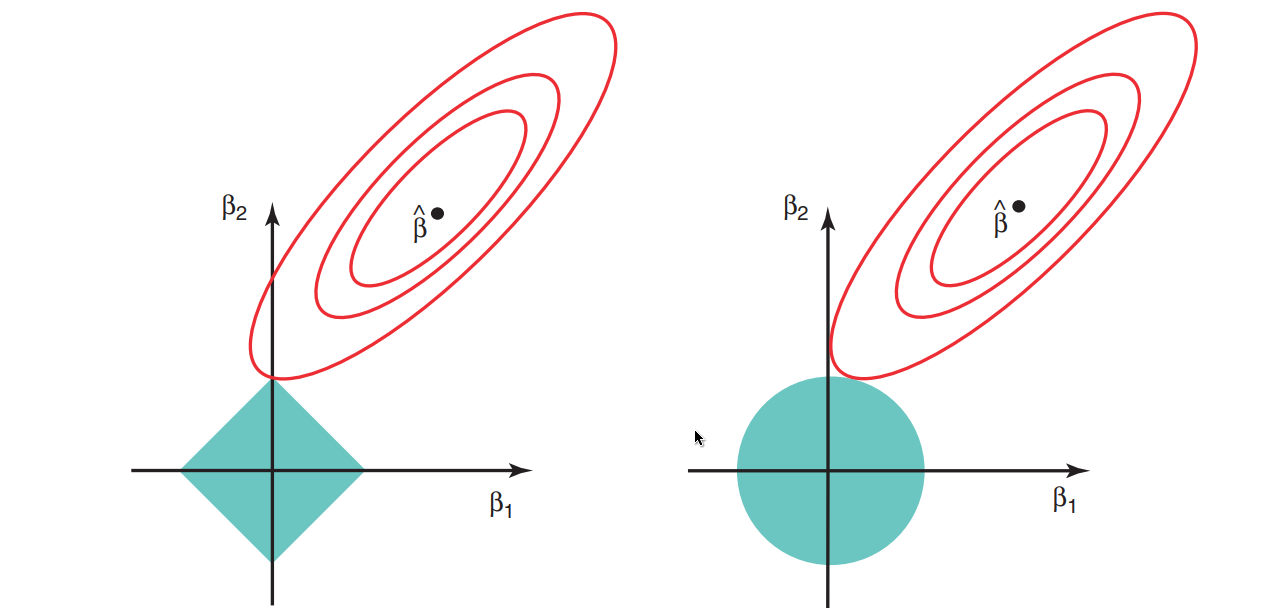
\includegraphics[width=1\linewidth]{Lasso_and_ridge.png}}
\caption{Границы ошибки $\sum_{i=1}^n(y_i - \sum_{j=1}^p \beta_j x_{ij})^2$ и ограничений  $\sum_{j = 1}^p |\beta_j| \leq ae$ для Лассо (слева) и $\sum_{j = 1}^p \beta_j^2 \leq \ae$ для гребневой регрессии (справа).}
\label{lasso_pic}
\end{figure}

\textbf{Замечания:}
\begin{itemize}
\item Обычно Лассо подходит лучше в случае наличия в данных большого количества лишних (незначимых) признаков.
\item Для реальных данных обычно заранее не известно количество признаков, значимо влияющих на зависимую переменную.
\item С помощью кросс-валидации можно определить какой подход лучше для конкретных данных.
\end{itemize}

\subsection{Elastic net regularization}
Решается задача оптимизации
\begin{equation*}
||Y-\mathbb{X}B||_{2}^{2} + \tau_{1}||B||_{1}^{2}+\tau_{2}||B||_{2}^{2}
\rightarrow\min_{B}.
\end{equation*}
\begin{itemize}
\item Elastic net --- это комбинация методов Lasso и Ridge:
\begin{itemize}
\item Когда $\tau_1 = 0$: Ridge регрессия;
\item Когда $\tau_2 = 0$: Lasso регрессия;
\end{itemize}
\item Elastic net обычно дает лучшие результаты, чем Lasso, при наличии коррелированных признаков;
\item При наличии группы релевантных и избыточных признаков Lasso обычно имеет тенденцию отказываться от всех, кроме одного признака из этой группы, в то время как Elastic net будет выбирать всю группу признаков.
\item Elastic net можно свести к SVM, для которого разработано много быстрых решений.
\end{itemize}

\section{Нелинейная регрессия}

 Пусть задана нелинейная модель регрессии $f(x,\theta)$, $\theta\in\mathbb{R}^{k}$.
 Решаем задачу минимизации функционала среднеквадратичного отклонения:
\begin{equation*}
Q(\theta,X)
=
\sum_{i=1}^{n}\left(
f(x_{i},\theta)-y_{i}
\right)^{2}
\to
\min_{B}.
\end{equation*}

К численному решению этой задачи можно применять метод стохастического градиента,  но он имеет первый порядок сходимости и может сходиться не слишком быстро. Далее рассмотрим методы второго порядка.

\subsection{Метод Ньютона-Рафсона}

Выберем начальное приближение $\theta^{0}=(\theta_{1}^{0},\ldots,\theta_{k}^{0})$ и организуем итерационный процесс
\begin{equation}\label{eq:iteration}
\theta^{t+1}:=
\theta^{t}
-
h_{t}(Q^{\prime\prime}(\theta^{t}))^{-1}Q^{\prime}(\theta^{t}),
\end{equation}
где $Q^{\prime}(\theta^{t})$ --- градиент $Q$ в точке $\theta^{t}$, $Q^{\prime\prime}(\theta^{t})$ --- гессиан $Q$ в точке $\theta^{t}$ (матрица порядка $k\times k$), $h_{t}$ --- величина шага (простейший вариант: $h_{t}=1$).

 Компоненты градиента:
\begin{equation}\label{eq:grad}
\frac{\partial Q(\theta)}{\partial \theta_{j}}
=
2\sum_{i=1}^{n}(f(x_{i},\theta)-y_{i})\frac{\partial f(x_{i},\theta)}{\partial \theta_j}.
\end{equation}

Компоненты гессиана:
\begin{equation}\label{eq:gessian}
\frac{\partial^{2} Q(\theta)}{\partial \theta_{j}\partial\theta_{m}}
=
2\sum_{i=1}^{n}
\frac{\partial f(x_{i},\theta)}{\partial\theta_{j}}
\frac{\partial f(x_{i},\theta)}{\partial\theta_{m}}
-
2\sum_{i=1}^{n}
(f(x_{i},\theta)-y_{i})
\frac{\partial^{2}f(x_{i},\theta)}{\partial\theta_{j}\partial\theta_{m}}.
\end{equation}


Основная сложность --- обращение гессиана (матрицы порядка $k\times k$) на каждой итерации \eqref{eq:iteration}. 

\subsection{Метод Ньютона-Гаусса}
Рассмотрим модификацию метода Ньютона-Рафсона, основанную на линеаризации функции $f$.

В методе Ньютона-Рафсона мы считаем градиент и гессиан в конкретных точках $\theta^{t}$. Можно считать, что в окрестности точки $\theta^{t}$ функция $f$ --- линейная.

 Линеаризация $f(x_{i},\theta)$ в окрестности $\theta^{t}$:
\begin{equation*}
f(x_{i},\theta)
=
f(x_{i},\theta^{t})
+
\sum_{j=1}^{k}
\frac{\partial f(x_{i},\theta_{j})}{\partial\theta_{j}}
(\theta_{j}-\theta_{j}^{t})
+
o(\theta_{j}-\theta_{j}^{t}).
\end{equation*}

 Подставляем это представление $f$ в формулы \eqref{eq:grad}, \eqref{eq:gessian}. Первые производные не изменятся, а вторые производные будут равны нулю. Таким образом избавились от второго слагаемого в формуле для компонент гессиана.
 
Введем обозначения:
\begin{itemize}
\item  $\mathbb{F}_{t}=(\frac{\partial f}{\partial\theta_{j}}(x_{i},\theta^{t}))_{n\times k}$ --- матрица первых производных,
\item  $f_{t}=(f(x_{i},\theta^{t}))_{n\times 1}$ --- вектор значений $f$.
\end{itemize}

Итерация метода Ньютона-Гаусса:
\begin{equation*}
\theta^{t+1}:=
\theta^{t}
-
h_{t}\underbrace{(\mathbb{F}_{t}^{\T}\mathbb{F}_{t})^{-1}\mathbb{F}_{t}^{\T}(f_{t}-Y)}_{\widetilde{B}}.
\end{equation*}

$\widetilde{B}$ --- решение задачи множественной линейной регрессии
\begin{equation*}
||\mathbb{F}_{t}B-(f_{t}-Y)||^{2}
\to
\min_{B}.
\end{equation*}

Таким образом нелинейная регрессия сводится к серии линейных регрессий.

\section{Приложение}
\subsection{Теорема Куна-Таккера}

Пусть $x\in\mathbb{R}^{n}$. Рассмотрим задачу 
\begin{gather*}
f(x)\to\min,\\
g_{i}(x)\leq 0,
\quad
i=0,\ldots,m.
\end{gather*}

\begin{theorem}\label{th:CT}
Пусть $f(x)$ выпукла и дифференцируема на допустимом множестве. Все ограничения регулярные (аффинные функции).
Тогда $x_{\ast}$ --- оптимальное решение тогда и только тогда, когда $\exists\lambda_{i}$ такие, что 
\begin{gather*}
\frac{\partial f(x_{\ast})}{\partial x_{j}}
+
\sum_{i=1}^{m}\lambda_{i}\frac{\partial g(x_{\ast})}{\partial x_{j}}=0
\quad
j=1,\ldots,n,\\
g_{i}(x_{\ast})\leq 0,\quad
\lambda_{i}\geq 0,
\quad
\lambda_{i}g_{i}(x_{\ast})=0,
\quad
i=1,\ldots,m.
\end{gather*}
\end{theorem}


\end{document}